\subsection*{Question 2.5}

If we compare figure \ref{fig:q25a} and \ref{fig:q25b}, it is clear
that the graphs are very are alike, but as can be seen in
figure \ref{fig:q25a} using the basis function $\phi(x) =
(1, \mathbf{x})$ makes the decision boundary between the two classes
linear and as can be seen from figure \ref{fig:q25b} using the basis
function $\phi(x) = (1, \mathbf{x}, \mathbf{x}^2)$ this results in a
hyperbola like decision boundary which we will also meet again
later. Overall the quadratic solution is better, but not by much.

\begin{figure}[!htbp]
  \centering
  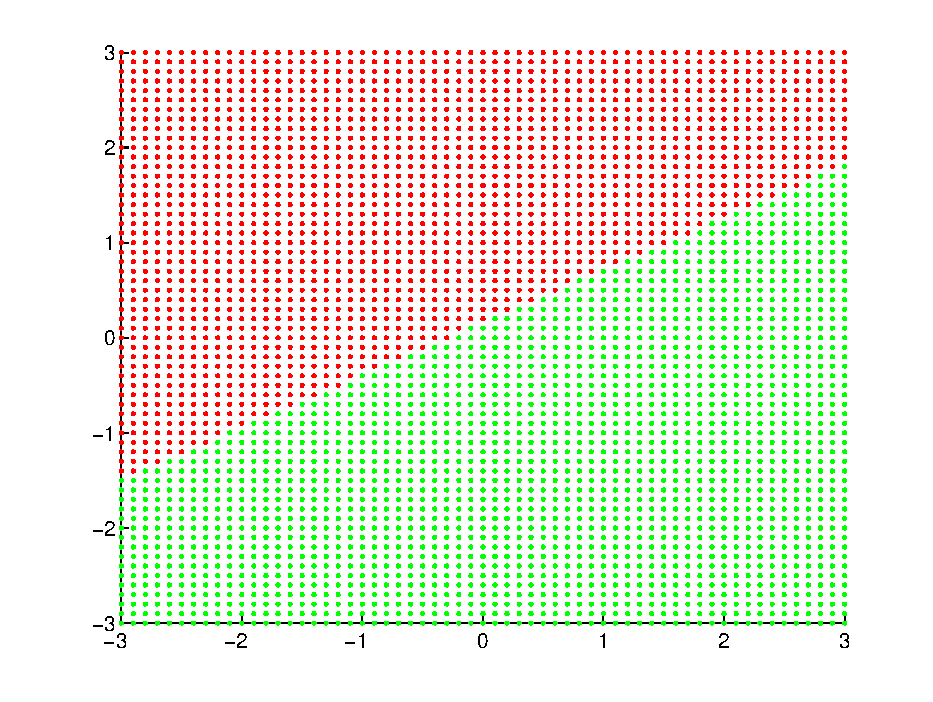
\includegraphics[width=0.6\textwidth]{./images/q25a.pdf}
  \caption{$\phi = (1,x)$, $N1 = 250$, $N2 = 250$}
  \label{fig:q25a}
\end{figure}

\begin{figure}[!htbp]
  \centering
  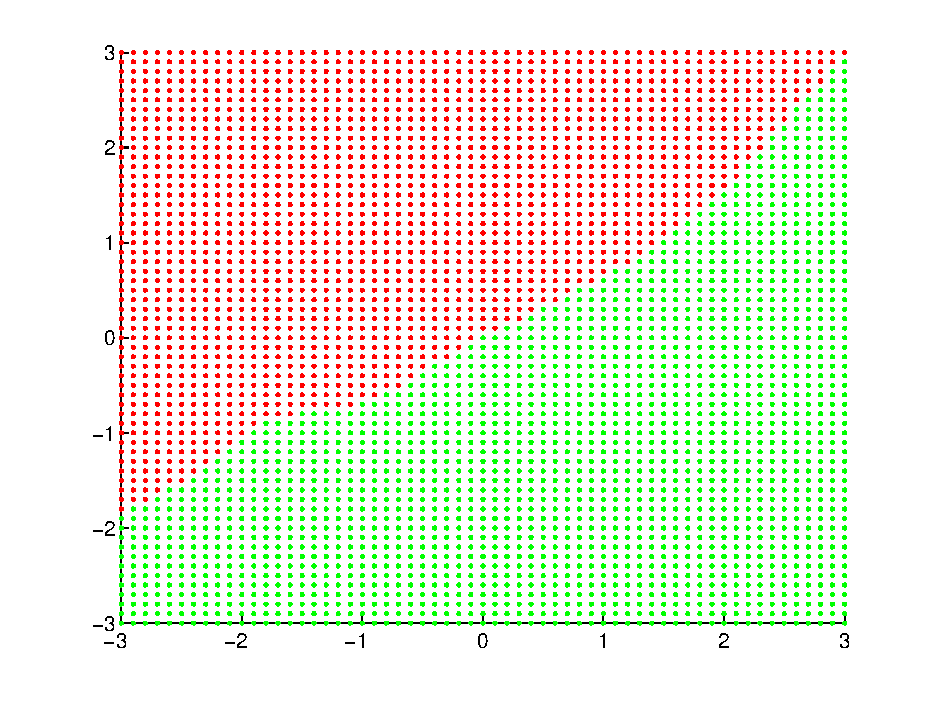
\includegraphics[width=0.6\textwidth]{./images/q25b.pdf}
  \caption{$\phi = (1,\mathbf{x}, \mathbf{x}^2)$, $N1 = 250$, $N2 = 250$}
  \label{fig:q25b}
\end{figure}
